\documentclass[10pt]{beamer}
\usetheme{pohan}
\usepackage{lipsum}
\usepackage{tabularx}
\usepackage{xcolor}
\usepackage{fancybox, graphicx}
\usepackage{animate}



\renewcommand{\arraystretch}{2}
\renewcommand\tabularxcolumn[1]{m{#1}}
\title{3/18 Paper Intro}
\subtitle{ + Paper Report Questions}
\author{Pohan Chi}
\date{\today}


\begin{document}

\maketitle

\maketoc


\section{SBERT-WK}

\begin{frame}{Title}
    \begin{figure}
        \begin{center}
            \shadowbox{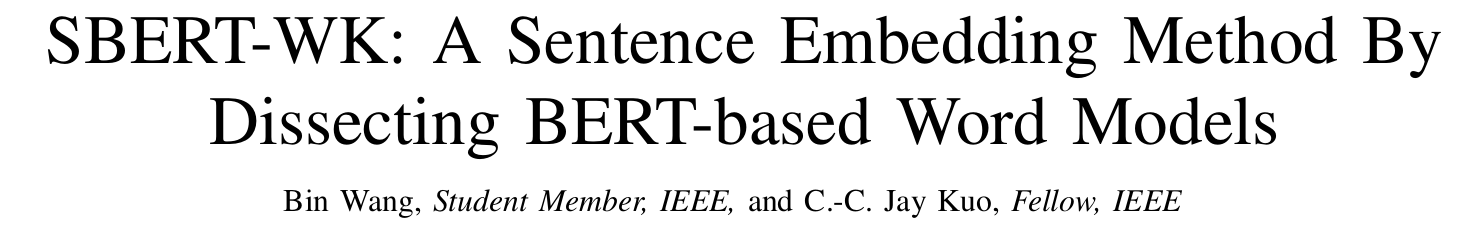
\includegraphics[width=0.95\textwidth]{img/SBERT-WK-title}}
        \end{center}
    \end{figure}
\end{frame}

\begin{frame}{SBERT-WK - Motivation}
    \begin{figure}
        \begin{center}
            \shadowbox{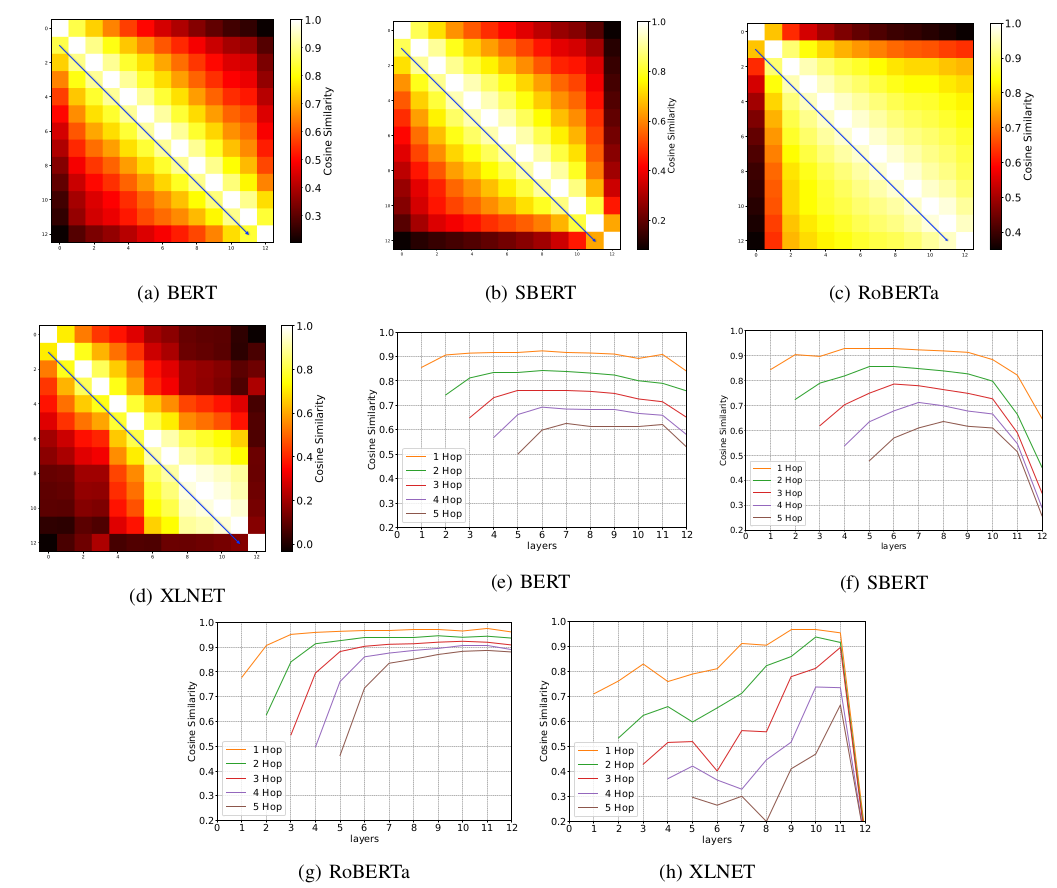
\includegraphics[height=0.7\textheight]{img/SBERT-motivation}}
        \end{center}
    \end{figure}
    
\end{frame}

\begin{frame}{SBERT-WK - Model}

    \begin{figure}
        \begin{center}
            \shadowbox{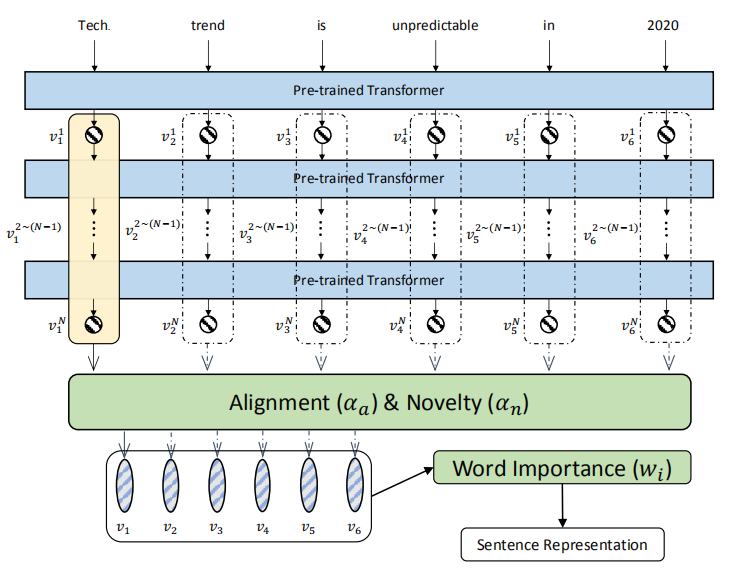
\includegraphics[width=0.8\textwidth]{img/SBERT-WK-model}}
        \end{center}
    \end{figure}

\end{frame}

\begin{frame}{SBERT-WK - Experiments}
    
    \begin{figure}
        \begin{center}
            \shadowbox{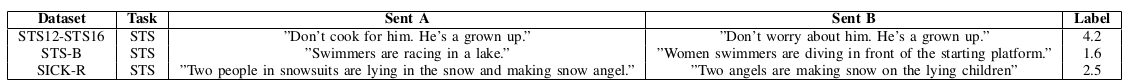
\includegraphics[width=0.97\textwidth]{img/dataset}}
        \end{center}
    \end{figure}

    \begin{figure}
        \begin{center}
            \shadowbox{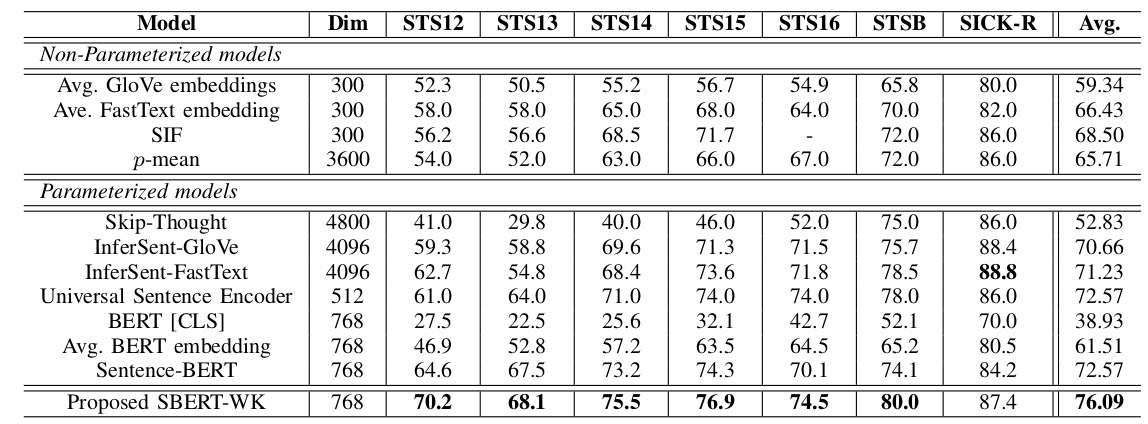
\includegraphics[width=0.95\textwidth]{img/sbert-wk-exp}}
        \end{center}
    \end{figure}

\end{frame}




\begin{frame}{SBERT-WK - Insight}

    \begin{enumerate}
        \item CLS token or averaging token embedding is good at Classification task but are not suitable for semantic textual similarity task.
        \item Connection between Cosine similarity and NSP task.
    \end{enumerate}

\end{frame}

\section{Mogrify LSTM}

\begin{frame}{Title}

    \begin{figure}
        \centering 
        \shadowbox{
\includegraphics[width=0.95\textwidth]{img/mogrifier}}
    \end{figure}

\end{frame}

\begin{frame}{Mogrify LSTM - Motivation}
    \begin{enumerate}
        \item Improve Generalization ability of Language Model
        \item Amplify salient and attenuate nuisance features in the input embeddings
        \item Context-free representation is a bottleneck in LM
        \item conditioning the input embedding on the recurrent state will improve performance. 
    \end{enumerate}
\end{frame}

\begin{frame}{Mogrify LSTM - Model}

    \begin{figure}
        \begin{center}
            \shadowbox{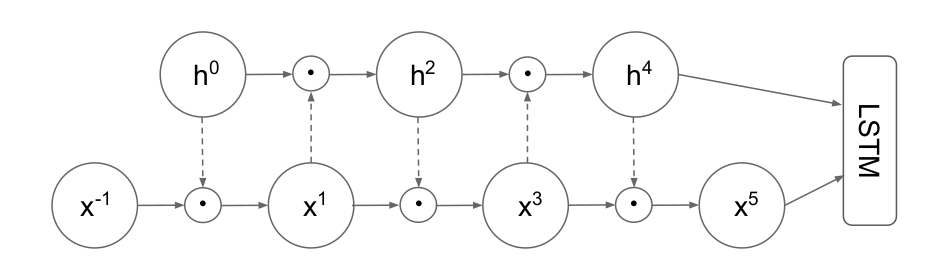
\includegraphics[width=0.95\textwidth]{img/mogrifier-model}}
            $$ x^i = 2 \sigma(Q^i h_{prev}^{i-1}) \odot x^{i - 2} \quad \text{for odd i in  [1,2,3,4..r]} $$
            $$ h^i_{prev} = 2 \sigma(R^i x^{i-1}) \odot h_{prev}^{i - 2}  \quad  \text{for even i in  [1,2,3,4..r]} $$

        \end{center}
    \end{figure}

\end{frame}

\begin{frame}{Mogrify LSTM - Experiments - (1)}

    \begin{figure}
        \begin{center}
            \shadowbox{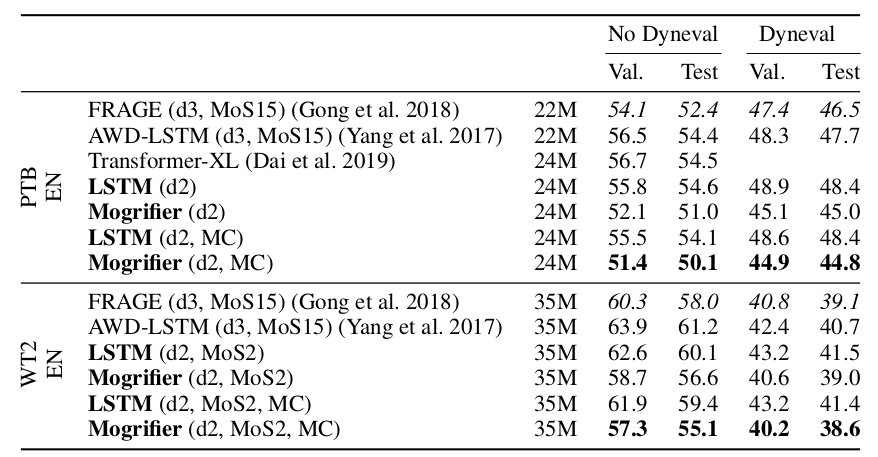
\includegraphics[width=0.95\textwidth]{img/mogrifier-exp}}
        \end{center}
    \end{figure}
\end{frame}

\begin{frame}{Mogrify LSTM - Experiments - (2)}
    
    \begin{figure}
        \begin{center}
            \shadowbox{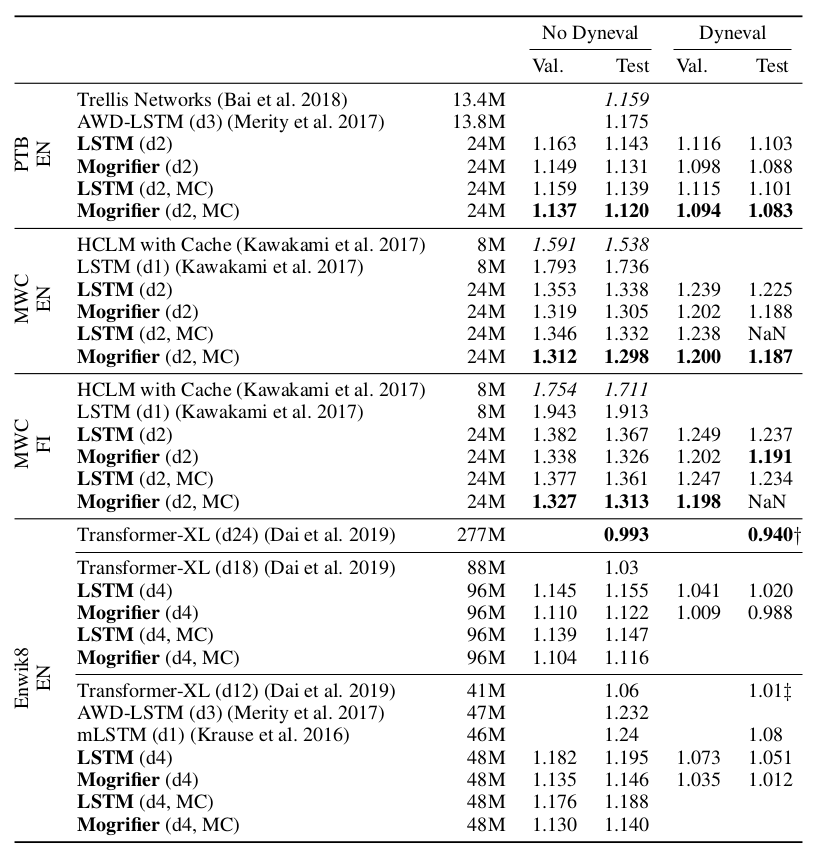
\includegraphics[width=0.6\textwidth]{img/Metric}}
        \end{center}
    \end{figure}

\end{frame}

\begin{frame}{Mogrify LSTM - Insight}
    \begin{enumerate}
        \item LSTM v.s Transformer
        \item another way to constrain LSTM input 
        \item Hypothesis
    \end{enumerate}
\end{frame}


\section{Retrospective Reader for Machine Reading Comprehension}

\begin{frame}{Title}
    \begin{figure}
        \begin{center}
            \shadowbox{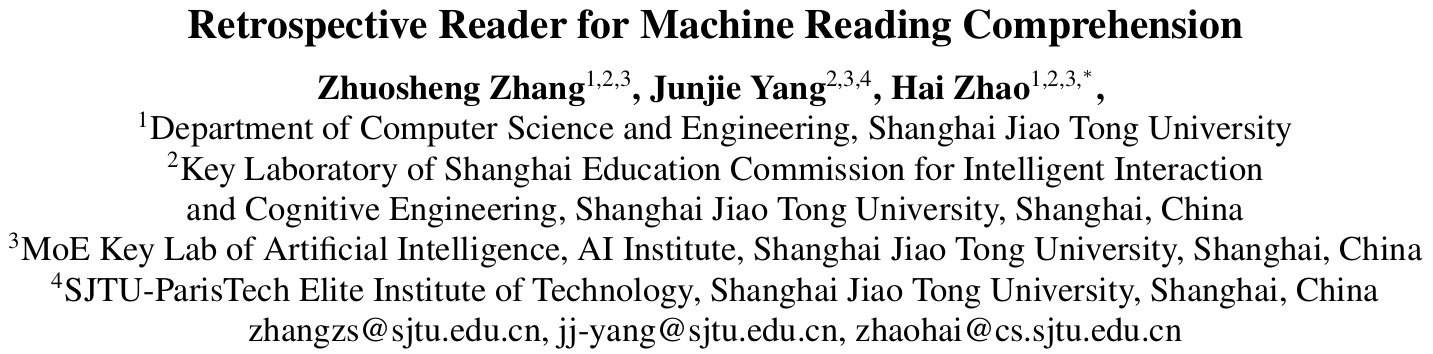
\includegraphics[width=0.95\textwidth]{img/Retrospective-Reader-title}}
        \end{center}
    \end{figure}
    
\end{frame}

\begin{frame}{Retrospective Reader - Motivation}
    
    Roberta, XLNet, ALBERT  - strong encoder !

    How about focus on Decoder ?
    \begin{figure}
        \begin{center}
            \shadowbox{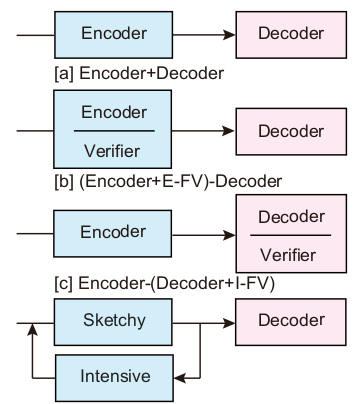
\includegraphics[height=0.6\textheight]{img/Retrospective-Reader-motivation}}
        \end{center}
    \end{figure}

\end{frame}

\begin{frame}{Retrospective Reader - Model}

    \begin{figure}
        \begin{center}
            \shadowbox{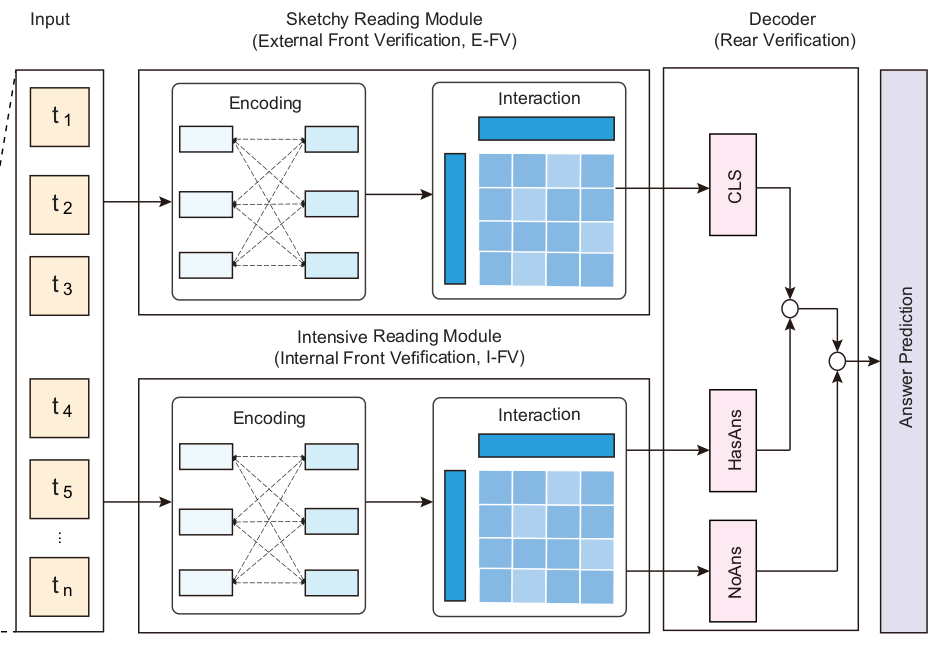
\includegraphics[height=0.75\textheight]{img/reader-overview}}
        \end{center}
    \end{figure}

\end{frame}

\begin{frame}{Retrospective Reader - Experiments}

    \begin{figure}
        \begin{center}
            \shadowbox{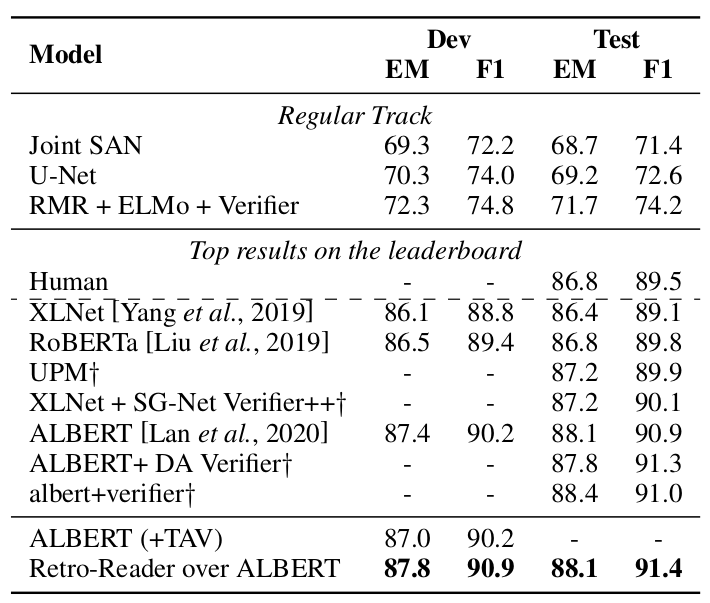
\includegraphics[height=0.75\textheight]{img/r2reader-experiment}}
        \end{center}
    \end{figure}

\end{frame}


\section{Differentiable Reasoning over a Virtual Knowledge Base}

\begin{frame}{Recap}
    \begin{figure}
        \begin{center}
            \shadowbox{\includegraphics[height=0.75\textheight]{img/Knowledge-base}}
        \end{center}
    \end{figure}
\end{frame}



\begin{frame}{Question 1}

    \begin{exampleblock}{What is the meaning of color in Table A ?}
    \end{exampleblock}

\end{frame}

\begin{frame}{Answer 1}

    \begin{exampleblock}{What is the meaning of color in Table A ?}
        Ans: 
        
        The matrices in the figures are just illustrations and not accurate in any sense. But A is an E x M matrix, and A[i, j] = 1 implies that entity i co-occurs with mention j, as set by the threshold in equation 3. Since a single entity can co-occur with multiple mentions, and a single mention can co-occur with multiple entities, both your interpretations are correct.
    \end{exampleblock}

\end{frame}

\begin{frame}{Question 2}

    \begin{exampleblock}{what is the initialization of z0 ? (one hot or k-hot vector)}
    \end{exampleblock}

\end{frame}

\begin{frame}{Answer 2}

    \begin{exampleblock}{what is the initialization of z0 ? (one hot or k-hot vector)}
        Ans: 

        We find a set of entities from the question and set them in z0. 
        
        In the case there is only 1 entity detected, it will be a 1-hot vector, otherwise it will be a k-hot vector.
    \end{exampleblock}

\end{frame}

\begin{frame}{Question 3}
    \begin{exampleblock}{z will be a one-hot vector or a k-hot vector after first round ?}
        
    \end{exampleblock}

\end{frame}


\begin{frame}{Ans 3}
    \begin{exampleblock}{z will be a one-hot vector or a k-hot vector after first round ?}
        Ans: Probabilities in each dimension.
    \end{exampleblock}

\end{frame}


\end{document}
